\documentclass[pdftex,12pt,letter]{article}
\usepackage{fancyhdr}
\usepackage{enumerate}
\usepackage{tabularx}
\usepackage{graphicx}
\usepackage{array}
\usepackage[justification=justified,singlelinecheck=false]{caption}
\usepackage{placeins}
\pagestyle{fancy}
\makeatletter
  \renewcommand\@seccntformat[1]{\csname the#1\endcsname.\quad}
\makeatother

\newcolumntype {Y}{ >{\raggedright \arraybackslash }X}
\newcommand{\HRule}{\rule{\linewidth}{0.5mm}}
\captionsetup{labelformat=empty}

\begin{document}

\begin{titlepage}
\begin{flushright}
\HRule \\[0.4cm]
{ \bfseries
{\huge Design Document\\[1cm]}
{\Large for\\[1cm]}
{\huge CWRUtility\large\\[4cm]}
{\large Prepared by\\Jason Kuster, Stuart Long, and William Ordiway\\[1cm]
Version 1.0 initial\\[1cm]
KOALAA Development\\[1cm]
October 6, 2012}}
\end{flushright}
\end{titlepage}
\tableofcontents{}
\begin{table}[!t]
\caption*{\bfseries Revision History}
\begin{tabularx}{\textwidth }[t]{|l|Y|Y|l|}
\hline
\bfseries Name & \bfseries Date & \bfseries Reasons for Change & \bfseries Version \\ \hline
Long & 10/6/2012 & Initial Outline & 1.0 initial\\
\hline
\end{tabularx}
\end{table}
\FloatBarrier
\newpage
\clearpage
\section{Overview}
\section{Features}
\subsection{Map}
The "Map" feature will allow the users to view a map of the Case Western Reserve University Campus. The feature will use the interactive map controller provided by the Windows Phone SDK. Since the map controller is already provided by the Windows Phone SDK, this feature will be very simple. It mostly just needs to send a saved map to the map controller and place the map controller on the screen.
\includegraphics[width=120mm]{MapDia.png}
\subsection{Schedule}
The "Schedule" feature will allow users to add classes or custom events to a saved schedule on the system. This feature will require three classes: a schedule event, a schedule event manager to handle schedule events, and a UI manager for the schedule.
\subsection{Class Diagram}
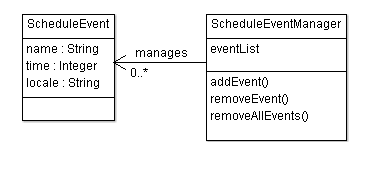
\includegraphics[width=80mm]{ScheduleEventsCD.png}
\figurename{Schedule Class Diagram}
\subsection{Class Descriptions}
The following class descriptions describe the above class diagram.
\subsubsection{ScheduleEvent}
\end{document}
